% Proseminar
% Sebastian Honegger
% FS15

\documentclass[9pt]{beamer}
\usetheme{Boadilla}  
\usepackage{wrapfig}				% Text umgibt Grafik


\title{Project Sihlstrasse}
%\subtitle{}
\institute[ETH Zurich] {Modelling and Simulating Social Systems\\ETH Zurich}

\author[Filip Meier and Sebastian Honegger]{Filip Meier and Sebastian Honegger}
\date{October 19, 2015}



\begin{document}

\begin{frame}
\frametitle{Traffic simulation Sihlstrasse}

\begin{figure}[H]
\begin{minipage}[t]{.20\textwidth}
\textbf{Leptonen:} $e\,\mu\,\tau\,\nu_e\,\nu_\mu\,\nu_\tau$ kommen frei in der Natur vor.\\
\textbf{Quarks:} $u\,d\,s\,c\,b\,t$ kommen nicht frei in der Natur vor.\\
Elementarteilchen werden aus Quarks aufgebaut: \textbf{Hadronen: Mesonen und Baryonen}\\
Mesonen: $\pi^+(u\overline{d})\,\pi^-(\overline{u}d)\,K^+(u\overline{s})\,K^-(\overline{u}s)$ \\
Baryonen: $p(uud)\, n(udd)\, \Lambda(uds)\, \Omega(sss)$
\end{minipage}\hfill
\begin{minipage}[t]{.25\textwidth}
	\centering
	\vspace{0pt}
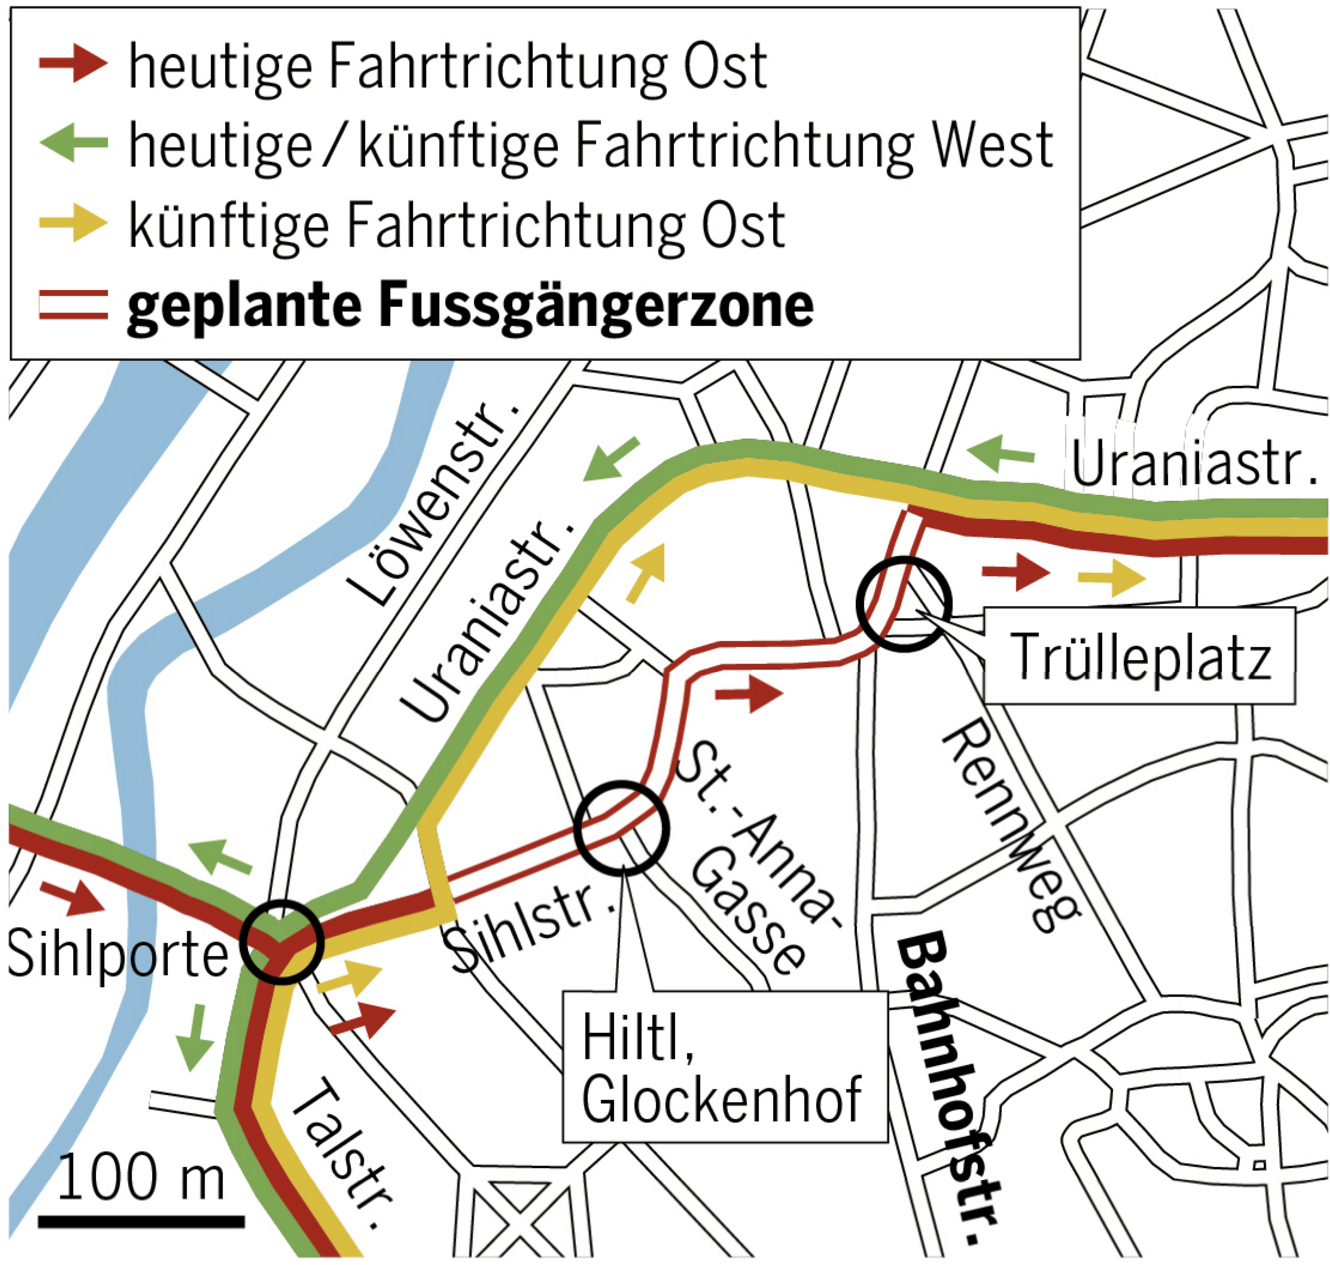
\includegraphics[width=\textwidth]{Plan_Sihlstrasse.png}
\end{minipage}\hfill
\end{figure}



\end{frame}



\end{document}





